\chapter{微正则系综}\label{ch:b3:microcanonical-ensemble}

一立方厘米空气中含有 $2.5\times10^{19}$ 个分子。
没有计算机能够积分它们的运动方程，
也没有实验能够给出初始条件——然而气体遵循
极其简洁的规律，而本科一年级分册中的热力学
从未提及一个分子，便已描述了它们。本章
搭建起一座桥梁：\emph{统计物理}，它从力学
加上严格的计数，推导出热的规律。
整座大厦建立在一条公设之上——孤立系统处于与其能量相容的
任一微观态的可能性相等——这一公设由
刘维尔定理奠定其合理性（
见\cref{ch:b3:hamiltonian-mechanics}）并借助
数量之巨大而变得强有力：当以
$10^{10^{20}}$ 为单位计数构型时，“压倒性可能”与“必然”
无从区分，概率凝结为规律。由计数可得熵、温度、压强
以及热力学第二定律——
并在本章末尾揭示橡皮筋为何回缩。

\section{微观态、宏观态与公设}

\begin{definition}[微观态与宏观态]\label{def:b3:microcanonical-ensemble:states}
\index{微观态}\index{宏观态}\index{微观态数}
\emph{微观态}是系统的完整微观描述，
即每个粒子的全部量子数（若按经典方法，
则为每个粒子的位置与动量，按相空间中体积 $h^3$ 的格子计数，
见\cref{prop:b3:schrodinger-three-dimensions:counting}）。
\emph{宏观态}是热力学所能观测的量：能量 $E$，
体积 $V$、粒子数 $N$、磁化强度\dots\ 
\emph{微观态数} $\Omega(E, V, N)$ 即具有同一宏观态的
微观态个数。
\end{definition}

\begin{theorem}[基本公设]\label{thm:b3:microcanonical-ensemble:postulate}
\index{微正则系综}\index{基本公设}
处于平衡态的孤立系统以相等的概率出现在
其 $\Omega(E, V, N)$ 个可及微观态中的每一个。平衡统计物理的全部内容
都由这一句话推出。
其依据在于：刘维尔定理表明，在能量壳层上的均匀分布
正是动力学所保持的分布——任何流动都不会使
相空间中的概率聚集——一个半世纪以来的
诸多推论从未与实验相悖。
\end{theorem}
\admitted

\begin{example}[$N$ 枚硬币组成的磁铁]\label{ex:b3:microcanonical-ensemble:spins}
$N$ 个相互独立的自旋，各自向上或向下，共 $2^N$ 个微观态。
宏观态“$n$ 个向上”的微观态数为 $\Omega(n) = \binom Nn$，
以压倒性优势在 $n = N/2$ 处取峰值，相对宽度
为 $\sim1/\sqrt N$。当 $N = 100$ 时，全部向上的态仅一个，
而均衡宏观态含 $\num{1e29}$ 个微观态。对于 $N = 10^{20}$，
即便向上比例的偏差只有 $10^{-8}$，也会被
$\eu^{-10^4}$ 之类的因子压低：系统\emph{正处于}其峰值，
而我们所说的平衡，即
微观态最多的宏观态。
\end{example}

\begin{omfigure}
\begin{tikzpicture}
  \begin{axis}[omaxis, axis x line=bottom, axis y line=left,
    width=11.4cm, height=5.4cm, xmin=0, xmax=1, ymin=0, ymax=1.15,
    xlabel={向上自旋的比例}, ylabel={概率（归一化）},
    xlabel style={at={(axis description cs:0.5,-0.1)}, anchor=north},
    xtick={0.25,0.5,0.75}, ytick=\empty, clip=false,
    legend style={font=\scriptsize, at={(0.03,0.95)}, anchor=north west,
      draw=none, fill=none}]
    \addplot[omExo, thick, domain=0:1, samples=120]
      {exp(-(x-0.5)^2*2*10)};
    \addlegendentry{$N = 10$}
    \addplot[omThm, thick, domain=0:1, samples=200]
      {exp(-(x-0.5)^2*2*100)};
    \addlegendentry{$N = 100$}
    \addplot[omDef, very thick, domain=0.3:0.7, samples=300]
      {exp(-(x-0.5)^2*2*3000)};
    \addlegendentry{$N = 3000$}
  \end{axis}
\end{tikzpicture}

{\small 自旋系统的微观态数随向上比例的变化，
对于增大的 $N$：峰值以 $1/\sqrt N$ 的速率变窄。在 $N \sim
10^{20}$ 时，“分布”在一切实际意义上只是
一个单一的值——宏观上的确定性
源于微观世界的“民主”。}
\end{omfigure}

\section{熵是一种计数}

\begin{definition}[玻尔兹曼熵]\label{def:b3:microcanonical-ensemble:entropy}
\index{熵!统计}
一个宏观态的\emph{统计熵}为
\[
S = k_{\text{B}}\ln\Omega , \qquad
k_{\text{B}} = \qty{1.38e-23}{J/K} .
\]
取对数后熵具有\emph{可加性}：微观态数
\emph{相乘}时，对于独立系统 $\Omega = \Omega_1\Omega_2$，
则 $S = S_1 + S_2$；玻尔兹曼常量使计数与
热力学早已选定的开尔文与焦耳单位相匹配。此
$S$ 将予以验证，即本科一年级分册中热力学第二定律的熵，
如今它具有微观含义：熵以对数
为计量单位，度量宏观态
可以\emph{通过多少种方式}实现。
\end{definition}

\begin{proposition}[理想气体的熵]\label{prop:b3:microcanonical-ensemble:gas}
\index{萨克尔–特特罗德公式}
计算置于箱中的 $N$ 个全同原子的量子态数
（见\cref{prop:b3:schrodinger-three-dimensions:counting}，每个原子在相空间中占一个
体积为 $h^3$ 的格子，并除以 $N!$ 以计入全同性——
见\cref{exo:b3:identical-particles:10}）得到
\[
S = Nk_{\text{B}}\Big[\ln\Big(\frac VN\,\frac1{\lambda_T^3}\Big)
 + \frac52\Big] , \qquad
\lambda_T = \frac{h}{\sqrt{2\pi mk_{\text{B}}T}}
\]
（\emph{萨克尔–特特罗德公式}；$\lambda_T$ 即热
德布罗意波长，是原子在
温度 $T$ 下的波包大小）。两项值得注意的检验：此式具有广延性
\emph{仅}借助 $N!$ 才成立；其绝对值——包括
$h$ 在内——与真实气体的量热熵相符
（见\cref{exo:b3:microcanonical-ensemble:11}）：经典
热力学在十九世纪的测量中，已经
在不自知的情况下认识了普朗克常量。
\end{proposition}
\admitted

\section{温度是计数的导数}

\begin{theorem}[平衡与温度]\label{thm:b3:microcanonical-ensemble:temperature}
\index{温度!统计定义}
设两个系统交换能量，总能量 $E = E_1 + E_2$ 固定。
联合微观态数 $\Omega_1(E_1)\,\Omega_2(E - E_1)$ 在
满足下式的划分处取最大值——且压倒性地如此——
\[
\frac{\partial S_1}{\partial E_1} =
\frac{\partial S_2}{\partial E_2} .
\]
定义
\[
\frac1T = \frac{\partial S}{\partial E}\bigg|_{V,N} ,
\]
平衡即\emph{温度相等}，能量会
自发地由高 $T$ 流向低 $T$，因为这一方向
使总计数增加。同样的逻辑用于体积与粒子交换，
得 $P/T = \partial S/\partial V$ 与 $-\mu/T
= \partial S/\partial N$：热力学中的全部强度量
都是计数的导数。
\end{theorem}

\begin{proof}
对 $\ln\Omega_1 + \ln\Omega_2$ 关于 $E_1$ 取极大值：驻定条件
即上文所述的等式。尖锐性方面，峰宽为
$\sim E/\sqrt N$（见\cref{exo:b3:microcanonical-ensemble:7}），故
极大值即为所观测到的态。若 $\partial S_1/\partial E_1 >
\partial S_2/\partial E_2$，则将能量\emph{移入}系统 1 会使
$S_{\text{总}}$ 增大：较冷的物体（$\partial S/\partial E$ 较大）
吸收能量——这即计数意义下热量由高温流向低温。
以理想气体验证：$S \propto \tfrac32 Nk_{\text{B}}\ln E + \cdots$
得 $1/T = \tfrac32 Nk_{\text{B}}/E$，即 $E = \tfrac32
Nk_{\text{B}}T$——即本科一年级分册中的气体动理论结果，
仅由纯粹的计数即可重新得到。
\end{proof}

\begin{omfigure}
\begin{tikzpicture}
  \begin{axis}[omaxis, axis x line=bottom, axis y line=left,
    width=11.2cm, height=5.2cm, xmin=0, xmax=1, ymin=0, ymax=1.2,
    xlabel={系统 1 的能量占比},
    ylabel={$\Omega_1\Omega_2$（归一化）},
    xlabel style={at={(axis description cs:0.5,-0.1)}, anchor=north},
    xtick={0.4}, xticklabels={$E_1^{\text{平衡}}$}, ytick=\empty, clip=false]
    \addplot[omDef, very thick, domain=0:1, samples=250]
      {exp(-(x-0.4)^2*900)};
    \node[omDef, font=\scriptsize, anchor=west] at (axis cs:0.47,0.75)
      {宽度 $\sim 1/\sqrt N$};
  \end{axis}
\end{tikzpicture}

{\small 两个共享能量的系统：联合计数随
划分的变化。平衡划分——即温度相等——不仅是
最可能出现的划分；对宏观 $N$ 而言，它
也是唯一被观测到的划分。}
\end{omfigure}

\section{热力学第二定律及更奇异的现象}

\begin{proposition}[不可逆性即计数]\label{prop:b3:microcanonical-ensemble:second-law}
\index{热力学第二定律!统计}
解除约束（移去隔板、打开阀门）只能
扩大可达的计数：$\Omega$ 增大，$S$ 增大——这正是
本科一年级分册中的第二定律，如今化为关于
概率的表述。逆过程并非被禁止，而是\emph{打折扣}：一团
由 $N$ 个分子组成的气体重新聚集到左半边的概率为
$2^{-N}$，而对于一立方厘米空气，其等待时间
超出宇宙年龄的倍数，其位数达 $10^{19}$ 位。
在此层次上，时间之箭
即计数增大的方向。
\end{proposition}

\begin{proof}[部分证明]
解除约束后，原本可达的每个微观态
仍然可达，并新增若干微观态：$\Omega$ 不会减小。
自由膨胀的计数：每个分子的可达体积加倍，
$\Omega \to 2^N\Omega$，于是 $\Delta S = Nk_{\text{B}}\ln2$——
恰与等温自由膨胀体积加倍的热力学结果一致。
\end{proof}

\begin{example}[负温度]\label{ex:b3:microcanonical-ensemble:negative}
\index{负温度}
能量\emph{有上界}的系统——即 $N$ 个自旋
置于磁场中，能量自 $-N\epsilon$ 至 $+N\epsilon$——其 $\Omega(E)$
先升后\emph{降}：越过平衡点后，再增加能量
反而使计数减少。此处 $\partial S/\partial E < 0$：
温度\emph{为负}。此类状态确实存在（粒子数
反转——即一切激光介质的工作状态——以及
通过磁场反转制备的自旋系统），它们并不冷，
而是\emph{比任何正温度都热}：能量由任何
$T < 0$ 的物体流入任何 $T > 0$ 的物体。温度的合理次序
为 $+0, \dots, +\infty \equiv -\infty, \dots, -0$：
$1/T$ 自然排出的次序，$T$ 却将其打乱
（见\cref{exo:b3:microcanonical-ensemble:9}）。
\end{example}

\begin{omfigure}
\begin{tikzpicture}
  \begin{axis}[omaxis, axis x line=bottom, axis y line=left,
    width=10.8cm, height=5.4cm, xmin=-1.05, xmax=1.05, ymin=0, ymax=0.78,
    xlabel={$E/N\epsilon$}, ylabel={$S/Nk_{\text{B}}$},
    xlabel style={at={(axis description cs:0.5,-0.1)}, anchor=north},
    xtick={-1,0,1}, ytick=\empty, clip=false]
    \addplot[omDef, very thick, domain=-0.999:0.999, samples=250]
      {-0.5*(1+x)*ln(0.5*(1+x)) - 0.5*(1-x)*ln(0.5*(1-x))};
    \node[font=\scriptsize, anchor=south] at (axis cs:-0.62,0.6)
      {$\partial S/\partial E > 0$: $T > 0$};
    \node[font=\scriptsize, anchor=south] at (axis cs:0.62,0.6)
      {$\partial S/\partial E < 0$: $T < 0$};
    \draw[gray, dashed] (axis cs:0,0) -- (axis cs:0,0.7);
    \node[font=\scriptsize, anchor=south] at (axis cs:0,0.71) {$T = \pm\infty$};
  \end{axis}
\end{tikzpicture}

{\small 双能级自旋系统的熵随能量变化。在
上升段温度为正；在峰顶温度
穿过无穷大；在下降段——粒子数反转——温度为负，
且比左侧任何状态都更“热”。}
\end{omfigure}

\begin{method}[微正则系综的计算要点]\label{met:b3:microcanonical-ensemble:method}
（1）列举：此处的微观态是什么，宏观态固定了什么？
（2）计数 $\Omega$——离散单元用组合计数，
气体则用相空间体积除以 $h^{3N}N!$。（3）尽早取对数：
斯特林公式（$\ln N! \approx N\ln N - N$）把
乘积化为易于处理的和。（4）对 $S$ 求导：能量的导数得到
$T$，体积的导数得到 $P$，粒子数的导数得到 $\mu$；
张力与场则用长度或磁化强度的导数求得
（\cref{pb:b3:microcanonical-ensemble:1}）。（5）相信峰值：
涨落按 $1/\sqrt N$ 减小，因此把“最可几”
换成“相等”，无需向任何人道歉。
\end{method}

\begin{omfigure}
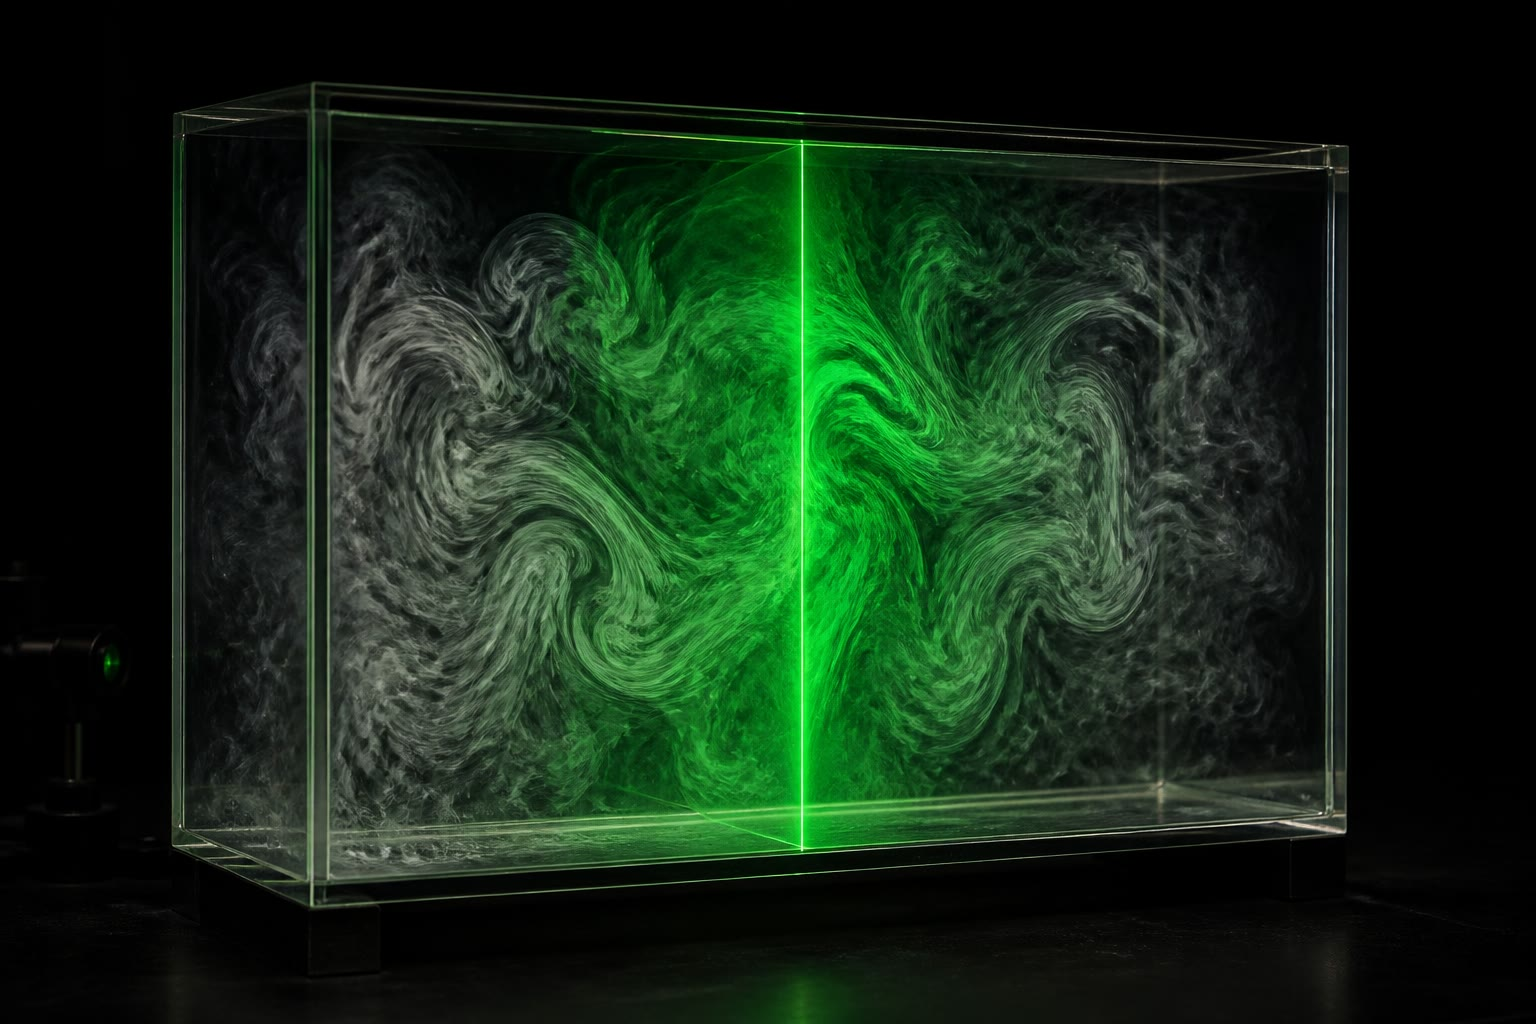
\includegraphics[width=0.58\linewidth]{images/book5/ai/b5-16-laser-sheet-smoke.jpg}

{\small 箱中被搅动的烟雾，被激光片切出一个截面：微观运动已超出任何逐项核算，统计规律接管了局面——力学问题变成熵问题的那一刻。}
\end{omfigure}

\section{练习}

\begin{exercise}[$\star$]\label{exo:b3:microcanonical-ensemble:1}
四个自旋。（a）列出各宏观态的重数 $\Omega(n)$，
此处宏观态即“$n$ 个向上”。（b）各宏观态在该假设下的概率。
（c）各宏观态的熵（以 $k_{\text{B}}$ 为单位）。
（d）哪一个宏观态是“平衡态”，以及“系统必定处于此态”这一
近似在 $N = 4$ 时到底有多粗糙？
\end{exercise}

\begin{exercise}[$\star$]\label{exo:b3:microcanonical-ensemble:2}
斯特林公式的实际应用。（a）比较 $\ln N!$ 与 $N\ln N - N$ 在
$N = 10$ 与 $N = 100$ 时的值（取 $\ln10! = 15.10$，$\ln100! = 363.7$）。
（b）证明相对误差按 $\ln N/N$ 的规律下降。（c）用斯特林公式
证明 $\ln\binom N{N/2} \approx N\ln2 - \tfrac12\ln N + $ 常数。
（d）为什么在一摩尔中略去 $\tfrac12\ln N$ 完全安全？
\end{exercise}

\begin{exercise}[$\star$]\label{exo:b3:microcanonical-ensemble:3}
（a）证明对两个独立系统有 $S = S_1 + S_2$。（b）若
某系统的 $\Omega$ 加倍，则 $S$ 增加多少——这一变化
对应单个粒子的哪种物理过程（\cref{prop:b3:microcanonical-ensemble:second-law}）？
（c）计算熵，
分别以 $k_{\text{B}}$ 和 J/K 为单位，求洗匀的一副 52 张扑克牌的熵
（取 $\ln52! \approx 156.4$）。（d）为什么牌的熵在热力学上
可以忽略，而分子的熵却不能？
\end{exercise}

\begin{exercise}[$\star$]\label{exo:b3:microcanonical-ensemble:4}
自由膨胀的核算。一摩尔气体向真空中膨胀，体积加倍。
（a）由计数论证求 $\Delta S$。（b）观察到气体
重新回到原来一半的概率。（c）估计
该类涨落的时间尺度，已知分子重排时间为
\qty{e-10}{s}——并与宇宙年龄
（\qty{4e17}{s}）比较。（d）热力学第二定律在何种确切意义上
“仅仅”是概率性的？
\end{exercise}

\begin{exercise}[$\star\star$]\label{exo:b3:microcanonical-ensemble:5}
理想气体的计数。从
$\Omega \propto \dfrac{V^N}{N!\,h^{3N}}\times$（动量壳层
体积 $\propto E^{3N/2}$）：（a）证明 $S = Nk_{\text{B}}[\ln V +
\tfrac32\ln E] - k_{\text{B}}\ln N! + $ 常数。（b）证明
若去掉 $N!$，把系统（$V$ 与 $N$ 同时）加倍，
则\emph{不会}使 $S$ 加倍——这正是
\cref{exo:b3:identical-particles:10}中所述的广延性失效。（c）用斯特林公式，把
结果写成 $S = Nk_{\text{B}}[\ln(V/N) + \tfrac32\ln(E/N)]
+ $ 常数 $\cdot N$。（d）哪些物理输入确定了历史上留下未定的两个
“常数”（量子胞大小；粒子
全同性）？
\end{exercise}

\begin{exercise}[$\star\star$]\label{exo:b3:microcanonical-ensemble:6}
由导数推导热力学关系。利用
\cref{exo:b3:microcanonical-ensemble:5}(c)的形式：（a）计算 $1/T =
\partial S/\partial E$，并还原 $E = \tfrac32 Nk_{\text{B}}T$；
（b）计算 $P/T = \partial S/\partial V$，并还原 $PV =
Nk_{\text{B}}T$；（c）导出绝热不变量：在
$S$ 与 $N$ 恒定时，证明 $VE^{3/2}$ 不变，即 $TV^{2/3}$ 不变——并
与本科一年级分册中的 $PV^{5/3}$ 相对照；（d）说明
已取得的成果：哪些经验定律刚刚
变成了计数的定理。
\end{exercise}

\begin{exercise}[$\star\star$]\label{exo:b3:microcanonical-ensemble:7}
平衡的尖锐性。两块相同的理想气体共享总
能量 $E$。（a）证明 $\ln[\Omega_1\Omega_2]$ 在
均分处取极大值。（b）对不平衡量 $x =
(E_1 - E_2)/E$ 作二阶展开，证明概率为
$\propto\eu^{-3Nx^2/4}$（每块有 $\tfrac32 N$ 个
自由度——系数不必精确）。（c）取 $N = 10^{22}$，求
方均根不平衡量。（d）该不平衡量所代表的温差
对应 \qty{300}{K} 下的气体：任何温度计能否测出
这一差值？
\end{exercise}

\begin{exercise}[$\star\star$]\label{exo:b3:microcanonical-ensemble:8}
双能级（肖特基）固体：$N$ 个格点，每个格点能量为 $0$ 或
$\epsilon$；$n$ 个被激发。（a）求 $\Omega(n)$ 与 $S(n)$。（b）令 $E =
n\epsilon$，利用斯特林公式，导出
\[
\frac1T = \frac{k_{\text{B}}}{\epsilon}\,
\ln\frac{N - n}{n} ,
\qquad\text{由此}\qquad
\frac nN = \frac{1}{\eu^{\epsilon/k_{\text{B}}T} + 1} .
\]
（c）画出 $E(T)$ 与热容的草图：一个凸峰（
\emph{肖特基反常}）出现在 $k_{\text{B}}T \sim \epsilon/2$ 附近——
为什么 $C$ 在两端都趋于零？（d）占据数公式的形式
曾在何处出现过，又将在何处再次出现
（\cref{ch:b3:quantum-statistics}）？
\end{exercise}

\begin{exercise}[$\star\star$]\label{exo:b3:microcanonical-ensemble:9}
负温度。对于
\cref{ex:b3:microcanonical-ensemble:negative}中的自旋系统，能级劈裂为
$\epsilon$：(a) 证明 $T < 0$ 当且仅当超过一半的自旋
朝上（粒子数反转）。(b) 对 60:40 的反转计算 $T$，
取 $\epsilon = \qty{e-4}{eV}$。(c) 证明能量总是从
负 $T$ 的物体流向正 $T$ 的物体（比较 $\partial
S/\partial E$）。(d) 为什么能量无界的系统（气体）
永远不能达到 $T < 0$？
\end{exercise}

\begin{exercise}[$\star\star\star$]\label{exo:b3:microcanonical-ensemble:10}
混合的定量分析。两种不同的气体（各含 $N$ 个分子，体积各为 $V$）
被连通。(a) 通过计数求 $\Delta S$。(b) 同一种气体：
计入 $N!$ 后，证明 $\Delta S = 0$。(c) 氦-3 与氦-4
不同：连通二者\emph{确实}会产生 $2Nk_{\text{B}}\ln2$
——但既无热量流动，也无做功：熵增加在物理上
体现在何处（若要重新分开它们，将付出什么代价）？(d)
在温度 $T$ 下重新分离所需的最小功：写出其表达式，并
说出建立在支付这笔代价之上的现代产业（同位素分离）。
\end{exercise}

\begin{exercise}[$\star\star\star$]\label{exo:b3:microcanonical-ensemble:11}
数表早就知道 $h$。用萨克尔–特特罗德公式计算氩气（$m =
\qty{6.6e-26}{kg}$）在 \qty{300}{K}、\qty{1}{bar}（$V/N =
k_{\text{B}}T/P$）：(a) 计算 $\lambda_T$；(b) 计算 $S/N
k_{\text{B}}$；(c) 与量热测得的值
$S_{\text{摩尔}} = \qty{154.8}{J/(mol.K)}$，即 $S/Nk_{\text{B}}
= 18.6$；(d) 说明所检验的内容：
哪两个量子输入包含在一个以冰量热计测得的
数值之中（1912 年以前）？
\end{exercise}

\begin{exercise}[$\star\star\star$]\label{exo:b3:microcanonical-ensemble:12}
能看见的涨落。气体中某一小块体积
$v$ 内分子数的涨落；相对偏差为 $\delta$ 的概率
$\propto\eu^{-\bar n\delta^2/2}$（$\bar n = Nv/V$——
可接受这一高斯分布，或由二项式推导）。(a) 设 $v$ 为
边长 \qty{550}{nm} 的立方体，处于大气密度下：求 $\bar n$ 与
方均根 $\delta$。(b) 为什么这些在光学尺度上永久存在的
千分之几的密度起伏，恰好就是
\cref{pb:b3:perturbation-theory:1} 所需要的，使空气得以散射
光？(c) 在多大的 $\bar n$（即多大的尺度）下，涨落
会达到 $10\%$？(d) 用一句话收束：天空的蓝色
正是关于 $\sqrt N$ 统计的一个陈述。
\end{exercise}

\section{问题：熵弹簧}

\begin{problem}[{周末问题——橡皮筋为何回拉}]\label{pb:b3:microcanonical-ensemble:1}
拉伸橡皮筋，它便弹回——然而其分子的
键几乎未变形，其内能也几乎不变。
橡胶的回复力并非寻求能量极小，而是
\emph{寻求熵的极大}：纯粹计数对力学机制的第一次大胜利，
同样的数学今日仍支撑
单分子 DNA 实验。模型：$N$ 个刚性连接段组成的链，
每段长 $b$，各自沿拉力轴指向左或右，
端到端伸长量 $x = (n_+ - n_-)\,b$。

\medskip\noindent\textbf{第一部分——计数构型。}
\begin{enumerate}
  \item 将 $n_\pm$ 用 $N$ 与 $x$ 表示，并写出
        微观态数 $\Omega(x)$。
  \item $\Omega$ 在何处取最大值？这对自由链的
        优选伸长量说明了什么？
  \item 利用斯特林公式，证明当 $x \ll Nb$ 时：
        \[
        S(x) \approx S(0) - \frac{k_{\text{B}}x^2}{2Nb^2} .
        \]
  \item 在此模型中，链的能量与 $x$ 无关：
        试论证为何可将任何回复力称为“熵性的”。
  \item 自由链的方均根伸长量为 $b\sqrt N$
        （随机游走）：对 $N = 10^4$ 与 $b = \qty{0.5}{nm}$，
        比较线团尺寸与拉伸后的长度 $Nb$。
  \item 实际橡胶是由此类链在
        交联点之间组成的网络：哪一个模型参数
        会因硫化（增加交联点）而改变？
\end{enumerate}

\medskip\noindent\textbf{第二部分——计数的力。}
\begin{enumerate}[resume]
  \item 对于温度为 $T$ 的系统，保持伸长量
        $x$ 所需的张力为 $f = -T\,\partial S/\partial x$，
        （可由 $\dd E = T\dd S + f\dd x$ 在定能条件下
        承认此式）：推导
        \[
        f = \frac{k_{\text{B}}T\,x}{Nb^2} .
        \]
  \item 胡克定律由此得出，劲度系数为 $k =
        k_{\text{B}}T/Nb^2$：对单条链，取 $N =
        \num{e4}$，$b = \qty{0.5}{nm}$，温度为 \qty{300}{K}，求其数值。
  \item 令人惊讶的因素是 $T$：橡皮筋
        在固定负载下\emph{被加热}时应当如何表现？与
        钢弹簧对比。
  \item 估算将一条链拉至其全长一半所需的力，
        以及力的尺度 $k_{\text{B}}T/b$，
        线性模型在该尺度下失效。
  \item 截面积为 \qty{1}{mm^2} 的橡皮筋中包含
        $\sim\num{e14}$ 条并联的有效链，估算其
        劲度系数，并与经验比较。
  \item 为什么橡胶随温度升高而变硬（而非变软），
        按每克计，而金属却变软？
\end{enumerate}

\medskip\noindent\textbf{第三部分——戈夫–焦耳厨房实验。}
\begin{enumerate}[resume]
  \item 将橡皮筋快速（绝热地）拉伸，并贴于
        嘴唇：它会变热。用熵的收支解释：拉伸
        \emph{减小}构型熵，因此在总量恒定的前提下
        熵（热量）须流向何处？
  \item 快速松开它：它会变冷。完成对称的
        论证。
  \item 挂有重物的橡皮筋被缓慢加热（用吹风机）：
        重物向哪个方向移动？为什么这是熵弹性的
        清晰标志？
  \item 设计用钢弹簧进行的对照实验：此时会
        发生什么变化？为何（属于哪一类弹性）？
  \item 一台热机：一个辐条为橡胶的轮子，一侧受热，
        稳定转动。追溯一个循环的逻辑（受热的辐条
        收缩，使轮子失去平衡）。
  \item 同一规律 $f = k_{\text{B}}Tx/Nb^2$ 由
        光镊对单个 DNA 分子测得（取 $b \approx
        \qty{100}{nm}$，$N \approx 500$，即细菌基因组
        片段），给出的力处于何种范围？（计算
        $k_{\text{B}}T/b$。）为什么这使该模型
        \emph{直接}可在单分子上检验？
\end{enumerate}

\medskip\noindent\textbf{第四部分——寓意。}
\begin{enumerate}[resume]
  \item 该链模型既无相互作用，也无能量标度，
        却给出一个力律：请精确指出这个力
        “来自”何处，
        并在本章的微正则语言中加以说明。
  \item 为什么力在 $T = 0$ 时消失？这说明
        在一个没有热运动的世界里，弹性的本质
        是什么？
  \item 比较熵弹性劲度系数对 $T$ 的线性关系与理想气体压强对 $T$ 的线性关系，
        证明二者是同一现象的不同表现：
        都是在约束条件下对构型计数，
        只是形式不同。
  \item 受热的带子提起重物，做了实际的功：追踪
        能量的来源与路径（从干燥机输入热量、熵的核算、
        输出功），并确认热力学第一定律
        未受影响。
  \item 理想链忽略了自回避效应与链的弯曲能。
        请分别说出每项省略所掩盖的橡胶的一个实测特征
        （接近完全伸长时的急剧变硬；
        应变诱导结晶与滞后）。
  \item 蛋白质折叠，膜发生涨落，聚合物卷曲：为什么
        体温下的 $k_{\text{B}}T$ 是所有软物质与生命物质通用的自然力单位
        （以皮牛顿计，即 $k_{\text{B}}T/\unit{nm}$，
        请算出它）？
  \item 概括这一有名的结论：一条由 $10^4$ 个无规连接的链段组成的链，
        若如实计数，便得到胡克定律，其中 $k =
        k_{\text{B}}T/Nb^2$，并预言橡胶被拉伸时会变热，
        受热时能提起重物——熵起着力的作用，
        这一点已从自行车内胎到单个 DNA 分子得到验证，
        力的尺度约为 $\sim\qty{0.04}{pN}$。
\end{enumerate}
\end{problem}
